\chapter{Syntax and Reduction Semantics}

\section{The syntax of lambda terms}
\label{sec:synlam}

The untyped lambda calculus has a very small syntax, an appealing
quality for both theoretical study and practical use.  There are just
two syntactic categories: variables and terms.  We assume variables
are taken from some countably infinite set of mathematical objects
(like the natural numbers) disjoint from the other forms of term, and
generally avoid specifying them further.  One stipulation, though is
that whatever variables are, we should be able to test effectively
whether or not two variables are equal.  Such an equality test will be
needed when defining substitution.  We will use $x$ as a meta-variable
for variables, and adopt the convention that in any particular
meta-linguistic discussion, different such meta-variables refer to
different variables.  So if we write $x$ and $y$, please understand
that these meta-variables refer to different actual variables.

Terms are then certain labeled binary trees.  We will use the
meta-variable $t$ (and decorated versions like $t_1$, $t'$, etc.) for
terms.  They are either leaf nodes labeled with variables $x$,
application nodes with subtrees $t_1$ and $t_2$, or lambda nodes with
subtree labeled $x$ and subtree $t'$.  Pictorially, these are shown in
Figure~\ref{fig:lamtrees}.  An application node is said to apply
$t_1$, as a function, to $t_2$, as an argument to that function.  For
a lambda node with subtree labeled $x$ and subtree $t'$, the term $t'$
is called the \emph{body} of the $\lambda$-node.  A term whose root is
labeled $\lambda$ is called a $\lambda$-abstraction.  

\begin{figure}
\begin{center}
\large
\begin{tikzpicture}
  \node at (0,0) {\ }
    child {node {$x$} edge from parent[draw=none]};

  \node at (3,0) {@}
  child { node {$t_1$}}
  child { node {$t_2$}};

  \node at (6,0) {$\lambda$}
  child { node {$x$}}
  child { node {$t'$}};

\end{tikzpicture}
\end{center}
\caption{Graphical depiction of the syntax of terms $t$}
\label{fig:lamtrees}
\end{figure}

While understanding the tree structure for terms is essential for the
study of lambda calculus, it is typical to present terms not as trees,
but textually.  For this, we use the following context-free
grammar, together with two parsing conventions:
\[
\textit{terms}\ t\ ::=\ x\ |\ t_1\ t_2\ |\ \lam{x}{t}\ |\ ( t )
\]
\noindent The parsing conventions are:
\begin{enumerate}
\item Application is left-associative.  So $a\ b\ c$ should be interpreted as $(a\ b)\ c$, as opposed to $a\ (b\ c)$.
\item The scope of $\lambda\ x$ is as far to the right as possible.  So $\lam{x}{x\ x}$ should be interpreted as $\lam{x}{(x\ x)}$, because this grouping shows that the $\lambda\ x$ part of the term governs the application $x\ x$.  This disambiguation is used, instead of $(\lam{x}{x})\ x$.
\end{enumerate}
\noindent Parentheses are just used for disambiguation and do not
correspond to any node in the tree syntax (of
Figure~\ref{fig:lamtrees}).  Figure~\ref{fig:exampleterms} shows
several example terms in both textual form and tree form.  Exercises
below (Section~\ref{sec:extree}) require you to translate between
these forms for some other examples.

\begin{figure}
\large
\begin{center}
\begin{tabular}{llll}

\underline{Textual:} &
$\lam{x}{x}$ &
$x\ \lam{x}{x\ x}$ &
$\lam{x}{\lam{y}{y\ x\ x}}$

\\ 
\underline{Disambiguated:} &
$\lam{x}{x}$ &
$x\ \lam{x}{(x\ x)}$ &
$\lam{x}{\lam{y}{((y\ x) x)}}$

\\ 

\begin{tikzpicture}
  \node at (0,0) {\underline{Tree:}}
  child { node {\ } edge from parent[draw=none]
    child { node {\ } edge from parent[draw=none]
      child { node {\ } edge from parent[draw=none]
        child { node {\ } edge from parent[draw=none]}}}};
\end{tikzpicture}

\vspace{1cm}
&

\begin{tikzpicture}
  \node at (0,0) {$\lambda$}
  child { node {$x$}}
  child { node {$x$}
    child { node {\ } edge from parent[draw=none]
      child { node {\ } edge from parent[draw=none]
        child { node {\ } edge from parent[draw=none]
}}}};
\end{tikzpicture}

&

\begin{tikzpicture}
  \node at (0,0) {@}
  child { node {$x$}}
  child { node {$\lambda$}
    child { node {$x$}}
    child { node {@}
      child { node {$x$} }
      child { node {$x$}
      child { node {\ } edge from parent[draw=none]}}}};
\end{tikzpicture}

&

\begin{tikzpicture}
  \node at (0,0) {$\lambda$}
  child { node {$x$}}
  child { node {$\lambda$}
    child { node {$y$}}
    child { node {@}
      child { node {@}
        child {node {$y$}}
        child {node {$x$}}}
      child { node {$x$}}}};
\end{tikzpicture}

\\


\end{tabular}

\end{center}
\caption{Some example terms, in textual form (where parsing conventions must be applied), then disambiguated textual form (no parsing conventions needed), and finally tree form}
\label{fig:exampleterms}
\end{figure}

\begin{definition}[subterm]
  A subterm of a term $t$ is just some subtree (possibly $t$ itself) of $t$.\index{subterm}
  \end{definition}

\section{Binding, bound, and free variable occurrences}

As will become more apparent shortly, the $\lambda$ symbol introduces
its variable $x$ \emph{locally} in the body.  This means that this $x$
used in the body of a $\lambda$-abstraction is semantically different
from the same variable $x$ used outside the body.  In Computer Science
terms, $\lambda$ introduces $x$ as a local variable, whose scope
(i.e., the part of the expression where this variable introduction is
in force) is the body of the $\lambda$-abstraction.

We have defined terms as certain finite labeled trees.  An occurrence of a variable $x$ in such a term
is a node of the tree that is labeled with $x$. The following basic terminology is then used for occurrences.

\begin{definition}[Binding occurrence]
  An occurrence of $x$ in $t$ is called binding iff it is
  the left child of a node labeled with $\lambda$.\index{variable!binding
  occurrence}
\end{definition}

\begin{definition}[Bound occurrence]
  An occurrence of $x$ in $t$ is called bound iff it occurs
  somewhere in the right subtree of a node $N$ labeled with $\lambda$,
  where the left child of $N$ is labeled $x$.\index{variable!bound occurrence}
\end{definition}

\begin{definition}[Free occurrence]
  An occurrence of $x$ in $t$ that is neither binding nor bound is called free.\index{variable!free occurrence}
\end{definition}


\noindent Figure~\ref{fig:varocc} gives examples of this terminology, for the term $(\lam{x}{x\ (x\ y)})\ (x\ y)$.

\begin{definition}[Free variable]
  A variable $x$ is free in $t$ iff it has a free occurrence in $t$.  The set of free variables of $t$ is denoted $\textit{FV}(t)$.
  \index{variable!free}\index{FV}.
\end{definition}

\noindent The free variables of the term shown in Figure~\ref{fig:varocc} are $x$ and $y$, because each of these has a free occurrence (boxed node) in the tree.

\begin{definition}[Open and closed terms]
A term with at least one free variable occurrence is called \emph{open}\index{term!open},
and a term with no free variable occurrences is called \emph{closed}\index{term!closed}.
\end{definition}

\noindent The term in Figure~\ref{fig:varocc} is open, because it has a non-empty set of free variables.  In contrast, the term $\lam{x}{x\ x}$ is closed, because its sole variable $x$ occurs only binding or bound.

\begin{figure}
\large
\begin{center}
    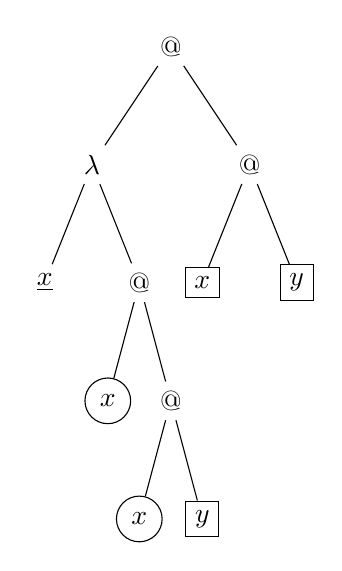
\begin{tikzpicture}
      [level 1/.style={sibling distance=20mm},
        level 2/.style={sibling distance=12mm},
          level 3/.style={sibling distance=8mm}]
      \node at (0,0) {@}
            child { node {$\lambda$}
              child { node {\underline{$x$}}}
              child { node {@}
                child { node [draw,circle] {$x$}}
                child { node {@}
                  child { node[draw,circle] {$x$}}
                  child { node[draw,rectangle] {$y$}}
}}}
            child { node {@}
              child {node[draw,rectangle] {$x$}}
              child {node[draw,rectangle] {$y$}}};
    \end{tikzpicture}
    \end{center}
    \caption{Example term illustrating the concepts of binding, bound, and free variable occurrence.  The underlined node is a binding occurrence, circled nodes are bound occurrences (bound by that sole underlined binding occurrence), and boxed nodes are free occurrences.}
    \label{fig:varocc}

\end{figure}

\section{Positions and subterms}
\label{sec:pos}

It is sometimes useful to be able to refer precisely to subterms of
terms, including variable occurrences, using \emph{positions}.  A
position $\pi$ is a finite sequence of $0$s and $1$s. Let us write
$\epsilon$ for the empty sequence, and $i\pi$ for the sequence that
begins with $i\in\{0,1\}$ and then continues with sequence $\pi$. Let
us elide $\epsilon$ in nonempty sequences. \index{position}

\begin{definition}[Subterm at a position]
  The subterm $t|_\pi$ of term $t$ at position $\pi$ is defined recursively by:
  \begin{eqnarray*}
    t|_\epsilon & = & t \\
    (t_0\ t_1)|_{i\pi} & = & t_i|_\pi \\
    (\lam{x}{t})|_{0} & = & x \\
    (\lam{x}{t})|_{1\pi} & = & t|_\pi
  \end{eqnarray*}
\end{definition}

For example, consider again the term $(\lam{x}{x\ (x\ y)})\ (x\ y)$ shown in Figure~\ref{fig:varocc}.  We have:
\begin{itemize}
  \item $((\lam{x}{x\ (x\ y)})\ (x\ y))|_{21} = (x\ y)|_1 = x|_\epsilon = x$
  \item $((\lam{x}{x\ (x\ y)})\ (x\ y))|_{11} = (\lam{x}{x\ (x\ y)})|_1 = x$
  \item $((\lam{x}{x\ (x\ y)})\ (x\ y))|_{122} = (\lam{x}{x\ (x\ y)})|_{22} = (x\ (x\ y))|_{2} = (x\ y)|_{\epsilon} = x\ y$
\end{itemize}

The subterm of $t$ at a position can be undefined, if the position extends beyond the leaves of tree $t$.  For example,
$((\lam{x}{x\ (x\ y)})\ (x\ y))|_{111}$ is undefined, because the position $111$ points past the binding occurrence of variable $x$.

\section{Capture-avoiding substitution}
\label{sec:subst}

To define how $\lambda$-terms compute (Section~\ref{sec:singlebeta}
below), we need a notion of substitution, where one term $t'$ is
substituted for the free occurrences of a variable $x$ in another term
$t$.  We will use the notation $[t'/x]t$ to denote the result of this
substitution, if defined\index{substitution!capture-avoiding}.
Substitution is used to define how lambda abstractions reduce (i.e.,
compute) when applied to arguments.  We will need to substitute
arguments $t'$ for input variables $x$ in bodies $t$ of
$\lambda$-abstractions.  Note that the notation $[t'/x]t$ is part of
our meta-language discussion of $\lambda$-calculus, and not new
object-language syntax within the language of $\lambda$-calculus.
Also, it should be mentioned that one finds numerous other notations
for substitution in the literature.  For example, Church writes
$\textsf{S}^x_{t'} t$ where we are instead writing $[t'/x]t$.

Defining substitution is, arguably, the central technical issue
in the definition of the lambda calculus.  The problem is essentially
one of the proper maintenance of scoping of variable, as we will
consider next.

\subsection{Variable capture}

 The main problem in defining substitution is to ensure that a
 substitution $[t'/x]t$ avoids \emph{variable capture}, where some
 free occurrences of a variable $y$ in the term $t'$ get captured by a
 $\lambda$-abstraction of $y$ occurring in $t$.  Such a capture would
 represent a change of scoping of those occurrences in $t'$: before
 the subsitution, they were not bound by any $\lambda$-abstraction in
 $t$, but after the substitution they are.  This change of scoping is
 to be prevented.

 The simplest example of the problem is $[y/x]\lam{y}{x}$.  A naive
 (and scope-incorrect) approach to substitution would produce $\lam{y}{y}$.
 But then the occurrence of $y$ that is being substituted has changed its scoping.  Before the
 substitution, it is not bound by the displayed $\lambda\ y$, but after the
 substitution, it is.  So it has been captured.

 It is common practice, in many research works, to deal with the
 problem of variable capture by assuming that variables are implicitly
 renamed to avoid capture.  So for this example, the common practice
 would be to say that the result of $[y/x]\lam{y}{x}$ is $\lam{w}{y}$,
 for some variable $w$ different from $x$ and $y$.  This is the
 approach taken in Hindley and Seldin's book, where it is even
 specified which variable $w$ (from the countably infinite supply of
 variables) is to be used~\cite{hindley+08}.  So substitution, in
 Hindley and Seldin, is indeed a function; not all authors are so
 careful.  Additionally, most works assume what is known as
 Barendregt's variable convention: in discussing some finite set of
 lambda terms, we assume that no variable occurs both free in one of
 the terms and bound in one of the terms~\cite[Definition
   2.1.13]{barendregt85}, and further assume that variables are
 implicitly renamed to ensure this.

 In this book, I will follow a different approach, adopting a modified
 version of Church's original proposal for dealing with renaming of
 variables~\cite{church41}.  During reduction, substitution is not
 allowed in case it would lead to capture, and variables must be
 explicitly renamed first in additional reduction steps.  I have
 several reasons for pursuing this approach.  First, as variable
 binding is one of the central technical issues of lambda calculus, it
 is better, certainly when first learning the theory, not too try to
 ignore the problem by assuming things are arranged so that it never
 arises.  Second, variable binding turns out to be one of the most
 tricky aspects both for implementation of languages incorporating
 lambda calculus, and for formalizing the meta-theory of such
 language in computer theorem-proving systems.  So again, dealing with
 the problem head-on seems best, as it may encourage development of the theory
 in a way that minimizes, rather than ignores, the issue.  Perhaps
 we will find better ways to formalize lambda calculus if we isolate
 the places where renaming is needed, for example.  And finally,
 some research is directly concerned with issues of renaming
 in lambda calculus, and thus needs to be completely explicit about
 the issue.  An example is works seeking to analyze when renaming
 can always be avoided~\cite{vanoostrom23}.


\subsection{Substitution as a partial function}

Figure~\ref{fig:subst} gives the definition of substitution as a
partial function.  Recall the meta-variable convention that $x$ and
$y$ are assumed to refer to different object-language variables.  In
Equations 3 and 4 it is intended (by the ``otherwise'' at the end of Equation 2)
that $x\in\textit{FV}(t_1\ t_2)$ and $x\in\textit{FV}(\lam{y}{t})$,
respectively.  This ensures that at most one equation can be
instantiated to obtain a fact about substitution $[t_1/x]t_2$, for any
particular $t_1$, $x$, and $t_2$.  For Equations 3 and 4, let us
understand that if the right-hand side of the equation is undefined
(in some instance of the equation), then the left-hand side is, too.

\begin{figure}
\large
\[
  \begin{array}{llll}
1. &    [t'/x]x & = & t' \\
2. &    [t'/x]t & = & t, \textnormal{if }x\not\in\textit{FV}(t); \textnormal{otherwise:} \\
3. &    [t'/x](t_1\ t_2) & = & ([t'/x] t_1)\ [t'/x]t_2 \\
4. &    [t'/x]\lam{y}{t} & = & \lam{y}{[t'/x]t}, \textnormal{if } y \not\in\textit{FV}(t')
  \end{array}
\]
  \caption{Recursive definition of capture-avoiding substitution as a
    partial function.  If a recursive call is undefined then the outer
    call is also considered undefined.  The case that is similar to
    the last clause of the definition but where $y\in\textit{FV}(t')$
    is the basic undefined case.  The clauses (equations) of the definition are numbered for reference later.}
  \label{fig:subst}
  \end{figure}

\subsection{Examples}

Here are some examples of capture-avoiding substitution.

\begin{enumerate}
\item $[\lam{x}{x}/y]\lam{z}{y\ z} = \lam{z}{(\lam{x}{x})\ z}$.  In detail, labeling the equality symbol with the number of the clause from Figure~\ref{fig:subst}, and underlining the part of the term that is being changed (just for clarity), the calculation is:

  \[
  \begin{array}{ll}
    \underline{[\lam{x}{x}/y]\lam{z}{y\ z}} & =_4 \\
    \lam{z}{\underline{[\lam{x}{x}/y](y\ z)}} & =_3 \\
    \lam{z}{\underline{([\lam{x}{x}/y]y)}\ [\lam{x}{x}/y]z} & =_1 \\
    \lam{z}{(\lam{x}{x})\ \underline{[\lam{x}{x}/y]z}} & =_2 \\
    \lam{z}{(\lam{x}{x})\ z} & \
  \end{array}
  \]

\item $[(x\ x)/y]\lam{y}{x\ y} = \lam{y}{x\ y}$.  This is just by clause 2 of Figure~\ref{fig:subst}, because we are substituting for variable $y$ in a $\lambda$-abstraction which binds $y$.  The $y$ for which we are substituting cannot possibly occur free in a $\lambda$-abstraction of $y$, so substitution stops, returning the term (into which we are trying to substitute) unchanged.

\item $[\lam{y}{x\ y}/z](z\ \lam{x}{x}) = (\lam{y}{x\ y})\ \lam{x}{x}$.  In detail, we have
  \[
    \begin{array}{ll}
      \underline{[\lam{y}{x\ y}/z](z\ \lam{x}{x})} & =_3 \\
      (\underline{[\lam{y}{x\ y}/z]z})\ [\lam{y}{x\ y}/z]\lam{x}{x} & =_1 \\
      (\lam{y}{x\ y})\ \underline{[\lam{y}{x\ y}/z]\lam{x}{x}} & =_2 \\
      (\lam{y}{x\ y})\ \lam{x}{x} & \ 
    \end{array}
    \]

  \item The substitution $[x\ x/y]\lam{x}{y\ y}$ is undefined, because
    to push the substitution inside a $\lambda$-abstraction, clause 4
    of Figure~\ref{fig:subst} requires that the $\lambda$-bound
    variable (in this case $x$) is not free in the term we are
    substituting (which here is $x\ x$).  Since $x$ is free in $x\ x$,
    this means we cannot apply any of the equations of Figure~\ref{fig:subst}
    and the substitution is undefined.
\end{enumerate}

\subsection{Some properties of capture-avoiding substitution}

The following lemmas are used below.  The proofs are a bit technical, carefully applying
the definition of substitution from Figure~\ref{fig:subst}.  Dealing with the possibility
that substitutions are undefined is a somewhat tedious necessity.  Each lemma is presented
with an example, before its proof.

\begin{lemma}
  If $t'$ is closed, then $[t'/x]t$ is defined.
\end{lemma}
\noindent\textit{Example.} $[\lam{x}{x}/x]\lam{y}{x\ y}$ is defined and equals
$\lam{y}{(\lam{x}{x})\ y}$.

\begin{proof}
  As $t'$ is closed, the condition in Equation 4 of Figure~\ref{fig:subst} can never
  be violated, and hence the substitution is defined.
\end{proof}

\begin{lemma}
\label{lem:substvargone}
  Suppose that $x\not\in\textit{FV}(t_1)$, and $[t_1/x]t_2$ is defined.  Then
  $x\not\in\textit{FV}([t_1/x]t_2)$.
\end{lemma}

\noindent\textit{Intuitive idea.} Substitution of a term $t_1$ for a variable $x$ in term $t_2$ results in a term
with no free occurrences of
$x$ (since they have all been replaced by substitution), as long as $x$ is not free in the substituted term $t_1$.

\vspace{.2cm}

\noindent\textit{Example.} Take $t_1$ to be $\lam{y}{y}$, and $t_2$ to be $x\ \lam{z}{z}$.
The conditions of the lemma are satisfied, and the result of applying the substitution
is $(\lam{y}{y})\ \lam{z}{z}$.  As stated in the lemma, $x$ does not occur free in this term.

\vspace{.2cm}

\noindent\textit{Example where the first condition does not hold.} If
we take $t_1$ to be $\lam{y}{x}$, and $t_2$ to be $x\ \lam{z}{z}$,
then the result of applying the substitution is
$(\lam{y}{x})\ \lam{z}{z}$, which does contain $x$ free.  Hence, the first condition is needed.

\begin{proof} The proof is by induction on $t_2$.
  If $x\not\in\textit{FV}(t_2)$, then by Equation 2 of Figure~\ref{fig:subst}, $[t_1/x]t_2 = t_2$, and
  hence $x\not\in\textit{FV}([t_1/x]t_2)$ (since $[t_1/x]t_2 = t_2$ and we are assuming $x\not\in\textit{FV}(t_2)$).
  So suppose $x\in\textit{FV}(t_2)$. If $t_2$ is $x$, then $[t_1/x]t_2 = t_1$,
  and the result follows by the assumption that $x\not\in\textit{FV}(t_1)$.
  If $t_2$ is $t_a\ t_b$ for some terms $t_a$ and $t_b$,
  then by the induction hypothesis, $x\not\in\textit{FV}([t_1/x]t_a)$ and $x\not\in\textit{FV}([t_1/x]t_b)$.
  So $x\not\in\textit{FV}([t_1/x](t_a\ t_b))$, since $[t_1/x](t_a\ t_b) = ([t_1/x]t_a)\ [t_1/x]t_b$ by Equation 3 of Figure~\ref{fig:subst}.
  If $t_2$ is $\lam{z}{t}$ for some $t$ and some $z$ different from $x$,
  then by the induction hypothesis, $x\not\in\textit{FV}([t_1/x]t)$.  So $x\not\in\textit{FV}(\lam{z}{[t_1/x]t})$.  The
  latter expression
    equals $[t_1/x]\lam{z}{t_2}$, since the substitution is assumed to be defined.
\end{proof}


\begin{lemma}
\label{lem:substundo}
  Suppose that $y\not\in\textit{FV}(t)$, and $[y/x]t$ is defined.  Then
  $[x/y][y/x]t$ is defined and equals $t$.
\end{lemma}

\noindent\textit{Intuitive idea.} Substituting variable $y$ for
variable $x$ and then reversing that (to substitute $x$ for $y$)
leaves the term unchanged, as long as it is legal to replace $x$ with
$y$ (avoiding capture), and as long as the original term does not have any free $y$ (since then substituting $x$ for $y$ would replace those free occurrences of $y$ with free occurrences of $x$, and the term would be different in the end).

\vspace{.2cm}

\noindent\textit{Example.} If we substitute $y$ for $x$ in $x\ \lam{x}{x}$, we get $y\ \lam{x}{x}$.  Then substituting $x$ for
$y$ restores the original term $x\ \lam{x}{x}$.

\begin{proof}
  The proof is by induction on $t$.  If $t$ is $x$, then $[x/y][y/x]x = x$.  If $x\not\in\textit{FV}(t)$,
  then $[x/y][y/x]t = [x/y]t$.  Furthermore, since $y\not\in\textit{FV}(t)$ by assumption, we have $[x/y]t = t$.
  For the rest of the proof, then, suppose $x\in\textit{FV}(t)$.

  If $t$ is $t_1\ t_2$ for some $t_1$ and $t_2$, then by the semantics of Figure~\ref{fig:subst},
  the expressions $[x/y][y/x](t_1\ t_2)$ and $([x/y][y/x]t_1)\ [x/y][y/x]t_2$ are either (a) both undefined
  or else (b) both defined and equal. Since $[y/x](t_1\ t_2)$ is defined, so are $[y/x]t_1$ and $[y/x]t_2$.
  By the induction hypothesis, then, $[x/y][y/x]t_1$ and
  $[x/y][y/x]t_2$ are defined and equal $t_1$ and $t_2$, respectively.  So $[x/y][y/x]t_1\ [x/y][y/x]t_2$ is defined and
  equals $t_1\ t_2$.  This means that it must have
  been option (b).  So $[x/y][y/x](t_1\ t_2)$ must be defined and equal to that same value, namely $t_1\ t_2$.

  Now suppose $t$ is a $\lambda$-abstraction of some variable different from $x$ (as the
  case where it is an abstraction of $x$ is covered above, by the reasoning when $x\not\in\textit{FV}(t)$).
  It is also not possible for $t$ to be $\lam{y}{t'}$ for any $t'$, because if the bound variable is $y$, the substitution
  $[y/x]\lam{y}{t'}$ is undefined, 
  So the only case we must consider is where $t$ is $\lam{z}{t'}$ for some $z$ (different from $x$ and $y$) and $t'$.

  We wish to apply the induction hypothesis to conclude that $[x/y][y/x]t'$ is defined and equals $t'$.  For this,
  we need to know first that $y\not\in\textit{FV}(t')$.  But this follows from the facts that $y\not\in\textit{FV}(\lam{z}{t'})$
  and $y \neq z$.  Second, we need to know that $[y/x]t'$ is defined.  But this follows since $[y/x]\lam{z}{t'}$ is
  defined and equals $\lam{z}{[y/x]t'}$.  Since that expression is defined, so also
  must its subexpression $[y/x]t'$ be defined.  So we can indeed apply the induction hypothesis to conclude
  that $[x/y][y/x]t'$ is defined and equals $t'$.

  Now again by the semantics of Figure~\ref{fig:subst}, since $z$ is different from $x$ and $y$, either $[x/y][y/x]\lam{z}{t'}$
  and $\lam{z}{[x/y][y/x]t'}$ are both undefined, or else both defined and equal.  But the reasoning of the previous
  paragraph shows that $\lam{z}{[x/y][y/x]t'}$ is defined (since we concluded that $[x/y][y/x]t'$ is defined)
  and equals $\lam{z}{t'}$ (since we concluded $[x/y][y/x]t' = t'$ by induction hypothesis).  Hence, $[x/y][y/x]\lam{z}{t'}$
  is also defined, and equals $\lam{z}{t'}$, as required.
\end{proof}

\section{Single-step beta-reduction}
\label{sec:singlebeta}

The central computational concept in $\lambda$-calculus is
\emph{$\beta$-reduction}, which explains how to evaluate function
calls.  A function call is an application of a $\lambda$-abstraction
to an argument.  So as a tree, it looks like:
\begin{center}
\begin{tikzpicture}
  \node at (0,0) {@}
  child { node {$\lambda$}
    child { node {$x$}}
    child { node {$t$} }}
  child { node {$t'$}};
\end{tikzpicture}
\end{center}
\noindent In textual form, it is $(\lam{x}{t})\ t'$.  The
$\beta$-axiom says that such a term reduces to $[t'/x]t$; i.e., the
result of substituting $t'$ for $x$ in
$t$, as discussed in Section~\ref{sec:subst} above.  This is only
allowed, however, if the substitution is defined.  Terms of the
form $(\lam{x}{t})\ t'$ are called
$\beta$-redexes (for ``$\beta$-reducible
expressions'')\index{$\beta$-redex}.  Operationally, this
reduction of the $\beta$-redex to the result of a substitution is
called \emph{contracting} the redex; the result of substitution is called
the \emph{contractum}
\index{$\beta$-redex!contracting}\index{contractum}.    Note that the requirement that
the substitution is defined is a particularity of the approach we take
in this book.

To give a formal definition of $\beta$-reduction, we will first define
what it means to reduce a single $\beta$-redex, and then, in
Section~\ref{sec:multibeta} below, define $\beta$-reduction with
multiple steps.  In both cases, we define relations between terms.  For
single-step $\beta$-reduction, the relation is denoted $\betar$.

You may recall that set theoretically, a relation is just a set of
ordered pairs, and we may equivalently write $(t,t')\in\betar$ or $t
\betar t'$ to indicate that $t$ $\beta$-reduces to $t'$.  There are
several ways to give the definition.
First, we can define the $\beta$-reduction relation using a set of inference rules\index{inference rule}.
Such rules are of the form
\[
\frac{\textit{premise}_1 \ \ \cdots \ \ \textit{premise}_n}{\textit{conclusion}}
\]
\noindent It is allowed for $n$ to be $0$, in which case there are no
premises and the rule is called an \emph{axiom}.  Inference rules are
to be understood as universally quantified implications: the
conjunction of the premises implies the conclusion, for all
instantiations of the meta-variables used.  A \emph{derivation} is a
kind of tree built by instantiating the inference rules in various
ways, and then using the conclusion of one inference as the premise of
another\index{derivation}.  Such instantiated inference rules are
called \emph{inferences}\index{inference}.  A derivation is
\emph{open} if there are some premises that are not the conclusion of
any inference\index{derivation!open}.  Otherwise, it is called
\emph{closed}\index{derivation!closed}. We further stipulate that we
are only interested in facts that can be proved using finite
derivations.  

A definition of $\beta$-reduction using inference rules is given in
Figure~\ref{fig:betar}.  The leftmost rule in the figure is the
$\beta$ rule, where we require that $[t'/x]t$ is defined
in order to use the rule for inferences in a derivation.  The other
three rules express the idea that a reduction can take place anywhere
in a term.  Figure~\ref{fig:betarex} gives some example derivations.
For some other examples:
\begin{itemize}
\item The term $(\lam{x}{x\ x})\ y$ single-step $\beta$-reduces to $y\ y$,
  using just the $\beta$ axiom.  This is because substituting $y$ for $x$
  in the body $x\ x$ of the $\lambda$-abstraction results in $y\ y$.
\item On the other hand, the term $(\lam{x}{\lam{y}{x}})\ y$ does not
  $\beta$-reduce, because the substitution $[x/y]\lam{y}{x}$, according
  to our definition of substitution, is undefined: replacing $x$ with $y$ in
  $\lam{y}{x}$ would result in variable capture.
  \end{itemize}
  
\begin{definition}[Single-step $\beta$-reduction (rules)]
\label{def:beta}
The relation $\betar$ is the set consisting of exactly those
pairs $(t,t')$ where $t \betar t'$ is derivable (via a finite derivation) using the
rules of Figure~\ref{fig:betar}.  We write applications of the
relation in infix notation (as in those rules).  If $t \betar t'$
we say that $t$ $\beta$-reduces to $t'$.  
\end{definition}

\begin{definition}[$\beta$-redex]
  Any term of the form $(\lam{x}{t})\ t'$ is called a $\beta$-redex.
  If $[t'/x]t$ is defined, let us call it a live $\beta$-redex.  Otherwise, let us call it
  a \emph{stuck} $\beta$-redex.\index{$\beta$-redex!stuck}\index{$\beta$-redex}\index{$\beta$-redex!live}
  \end{definition}

\begin{definition}[nested redex]
  Suppose that a redex $R_1$ is a subterm of some other redex $R_2$.
  Then we say that $R_1$ is a nested redex (nested within $R_2$).
  \end{definition}
 
\begin{definition}[$\beta$-expansion]
\label{def:betaexpand}
  The inverse of the $\leadsto_\beta$ relation is called
  $\beta$-expansion.  If $t \leadsto_\beta t'$, we say
  that $t'$ $\beta$-expands to $t$.\index{$\beta$-expansion}
\end{definition}

\begin{figure}
  \[
  \begin{array}{lllllll}
\infer{(\lam{x}{t})\ t'\ \betar\ [t'/x]t}{\ } & \ &
\infer{\lam{x}{t}\ \betar\ \lam{x}{t'}}{t\ \betar\ t'} & \ &
\infer{t_1\ t_2\ \betar\ t_1'\ t_2}{t_1\ \betar\ t_1'} &\ &
\infer{t_1\ t_2\ \betar\ t_1\ t_2'}{t_2\ \betar\ t_2'}
  \end{array}
  \]
  \caption{Inference rules defining the $\beta$-reduction relation.  It is required that the substitution in the leftmost rule be defined, in order to use the rule.}
  \label{fig:betar}
\end{figure}

\begin{figure}
  \[
  \begin{array}{lll}
    \infer{(\lam{x}{x\ x})\ \lam{y}{y} \betar (\lam{y}{y})\ \lam{y}{y}}
          {\ }
    &
    \infer{\lam{x}{(\lam{y}{y})\ x} \betar \lam{x}{x}}
          {\infer{(\lam{y}{y})\ x \betar x}{\ }}

    &

    \infer{x\ (y\ ((\lam{x}{x})\ z)) \betar x\ (y\ z)}
          {\infer{y\ ((\lam{x}{x})\ z) \betar y\ z}
            {\infer{(\lam{x}{x})\ z \betar z}{\ }}}
  \end{array}
\]
\caption{Example derivations using the rules of Figure~\ref{fig:betar} for $\beta$-reduction.}
\label{fig:betarex}
\end{figure}

\noindent The following definition is generic, for any $R\subseteq (A\times A)$.  We will call such
a set a (binary) relation on $A$.\index{binary relation on a set}

\begin{definition}[determinism]
\label{def:det}
  An element $x$ is said to be deterministic with respect to some
  relation $R$ on a set $A$ iff for all $y$ and $y'$, if $x R y$ and
  $x R y'$ then $y = y'$.  $R$ itself is called deterministic iff
  every element of $A$ is deterministic with respect to $R$.
  Mathematically, being deterministic is the same as being a
  functional relation.  A nondeterministic relation is then simply one
  which fails to be deterministic for at least one
  $x$.\index{relation!deterministic}\index{determinism}
  \end{definition}

\begin{lemma}
  The $\leadsto_\beta$ relation is nondeterministic.
\end{lemma}
\begin{proof}
  Any term containing two non-nested $\beta$-redexes will have
  two distinct contracta.  For example, $(\lam{x}{x}\ y)\ (\lam{x}{x}\ z)$
  has distinct contracta $y\ (\lam{x}{x}\ z)$ and $(\lam{x}{x}\ y)\ z$.
  Hence, $\leadsto_\beta$ is nondeterministic.
\end{proof}

\subsection{An alternative definition using contexts}

Another way to define the same $\betar$ relation is with
contexts.  Let us first introduce the concept of \emph{grafting},
which is just substitution that does \underline{not} avoid
capture\index{grafting}.  We will write $\langle t/x\rangle t'$ for
the grafting relation (there does not seem to be a generally adopted
notation for grafting).  The definition, given in
Figure~\ref{fig:grafting}, is essentially the same as the one for substitution,
except that the last clause does not impose
any requirements on $\textit{FV}(t')$.

\begin{figure}
\large
\[
  \begin{array}{lll}
\    \langle t'/x \rangle x & = & t' \\
\    \langle t'/x \rangle t & = & t, \textnormal{if }x\not\in\textit{FV}(t); \textnormal{otherwise:} \\
\    \langle t'/x \rangle(t_1\ t_2) & = & (\langle t'/x\rangle t_1)\ \langle t'/x\rangle t_2 \\
\    \langle t'/x\rangle\lam{y}{t} & = & \lam{y}{\langle t'/x\rangle t}
  \end{array}
\]
  \caption{Recursive definition of grafting, a total function similar to substitution but intentionally allowing variable capture.}
  \label{fig:grafting}
  \end{figure}

\begin{definition}[context]
  A term $t$ is called a context iff it contains exactly one free
  occurrence of a special fixed variable $q$\index{context}.  If $t$
  is a context, then we write $\langle t'/q \rangle t$ more briefly as
  $\langle t' \rangle t$.  The variable $q$ is called the hole of the
  context\index{context!hole}.
  \end{definition}

\noindent Using contexts, we may give the following alternative definition of the $\beta$-reduction relation:

\begin{definition}[Single-step $\beta$-reduction (contexts)]
\label{def:betactxt}
The single-step $\beta$-reduction relation
$\betar$ is alternatively defined to be the set of all ordered pairs with first component $\langle (\lam{x}{t})\ t' \rangle t''$
  and second component $\langle [t'/x]t \rangle t''$, for some $x$, $t$, $t'$, and $t''$ (with $t''$ a context and $[t'/x]t$ defined).
\end{definition}

The idea of this definition is to express that (in operational terms)
if you find a $\beta$-redex somewhere in some possibly bigger term
$t_1$, then you may reduce $t_1$ by contracting that $\beta$-redex and
then rebuilding the rest of the term $t_1$ around the contractum.  The
definition expresses finding $(\lam{x}{t})\ t'$ in possibly bigger
term $t_1$ by writing $\langle(\lam{x}{t})\ t'\rangle t''$ for $t_1$.
In other words, you have some term $t_1$ that contains a designated
occurrence of the redex, because $t_1$ is what you get when you graft
the redex in for the single occurrence of special variable $q$ in some
context $t''$.  The reason that we use grafting for this definition
instead of substitution is to allow contraction of redexes that
contain free variables that are bound in $t_1$.  We will discuss this
point further in the examples next.

\subsubsection{Examples}
\label{sec:betaex}

\begin{enumerate}
  \item $(\lam{x}{x\ x})\ \lam{y}{y}$ reduces to
    $(\lam{y}{y})\ \lam{y}{y}$.  For this, the meta-variables of
    Definition~\ref{def:betactxt} are instantiated thus:
    \begin{itemize}
    \item $x$ is instantiated with $x$,
    \item $t$ with $x\ x$,
    \item $t'$ with $\lam{y}{y}$
    \item $t''$ with $q$ (the special context variable)
    \end{itemize}

\item $\lam{x}{(\lam{y}{y})\ x}$ reduces to $\lam{x}{x}$.  Here the instantiations for Definition~\ref{def:betactxt} are:
    \begin{itemize}
    \item $x$ is instantiated with $y$,
    \item $t$ with $y$,
    \item $t'$ with $x$
    \item $t''$ with $\lam{x}{q}$.
    \end{itemize}

    Notice that here we really need the idea of grafting, because our
    redex contains $x$ free, which is bound in $t''$.  We want to
    allow reduction of redexes that contain variables bound outside
    the redex, and so we use grafting to specify that the $x$ in the
    redex may be bound in $t''$.  If we used substitution instead of
    grafting, this reduction would not be allowed by
    Definition~\ref{def:betactxt}, because $[(\lam{y}{y})\ x/q]\lam{x}{q}$
    is undefined (as the $x$ in $(\lam{y}{y})\ x$ would be captured
    pushing the substitution into $\lam{x}{q}$).

  \item $(\lam{x}{x\ x})\ \lam{x}{x\ x}$ reduces to that very same term.  The instantiations for Definition~\ref{def:betactxt} are:
    
    \begin{itemize}
    \item $x$ is instantiated with $x$,
    \item $t$ with $x\ x$,
    \item $t'$ with $\lam{x}{x\ x}$
    \item $t''$ with $q$.
    \end{itemize}

    We calculate the substitution $[t'/x]t$ as follows (referencing clause numbers from Figure~\ref{fig:subst}):
    \[
    \begin{array}{ll}
      \underline{[\lam{x}{x\ x} / x](x\ x)} & =_3 \\
      (\underline{[\lam{x}{x\ x} / x]x})\ [\lam{x}{x\ x} / x]x & =_1 \\
      (\lam{x}{x\ x})\ \underline{[\lam{x}{x\ x} / x]x} & =_1 \\
      (\lam{x}{x\ x})\ \lam{x}{x\ x} & \ 
    \end{array}
    \]
    \noindent This is an important basic example, because it shows
    that terms can reduce to themselves, and hence can give rise to
    infinite reductions (to be defined just below).
    \end{enumerate}

\subsection{One more alternative: replacement at a position}

Yet one further alternative definition of single-step $\beta$-reduction
is using the notion of replacement of a subterm at a position.

\begin{definition}[Replacement at a position]
  The term $t[t']_\pi$ replacing the subterm of $t$ at position $\pi$ by $t'$ is defined recursively by:
  \begin{eqnarray*}
    t[t']_\epsilon & = & t' \\
    (t_1\ t_2)[t']_{1\pi} & = & (t_1[t']_\pi)\ t_2 \\
    (t_1\ t_2)[t']_{2\pi} & = & t_1\ (t_2[t']_\pi) \\    
    (\lam{x}{t})[t']_{2\pi} & = & \lam{x}.(t[t']_\pi)
  \end{eqnarray*}
\end{definition}

\noindent For an example:
\[
\begin{array}{ll}
  (\lam{x}{\lam{y}{x\ y}})[y\ \lam{z}{z}]_{22} & = \\
  \lam{x}{((\lam{y}{x\ y})[y\ \lam{z}{z}]_{2})} & = \\
  \lam{x}{\lam{y}{((x\ y)[y\ \lam{z}{z}]_{\epsilon})}} & = \\
  \lam{x}{\lam{y}{(y\ \lam{z}{z})}}
\end{array}
\]
Note that replacement of binding occurrences of variables is not allowed by this definition.

Using replacement, we can give yet another definition for single-step $\beta$-reduction:

\begin{definition}[Single-step $\beta$-reduction (replacement at position)]
\label{def:betapos}
The single-step $\beta$-reduction relation
$\betar$ is alternatively defined to be the set of all ordered pairs with first component $t''[(\lam{x}{t})\ t']_\pi$
and second component $t''[[t'/x]t]_\pi$, for some $x$, $t$, $t'$, $t''$, and $\pi$, where $\pi$ is a legal position of $t''$
and $[t'/x]t$ defined.
\end{definition}

This definition uses a position to name where a $\beta$-redex is to be found and contracted, instead of using the hole of a context
to show where the contraction takes place.

\section{Definitions using closure operators}
\label{sec:clos}

In what follows, yet another way of defining single-step
$\beta$-reduction will prove illuminating, which is via
\textbf{closure operators} on relations.\index{closure operator}
Such an operator takes a relation $R$ and produces some new relation (let us
call it $R'$) such that $R\subseteq R'$ and $R'$ satisfies some desired property.
We will generally define closure operators using rules.

An important example in our setting is the \textbf{compatible closure},
which we will denote
$\Tau[R]$, of $R$. \index{compatible closure} The rules for this are
given in Figure~\ref{fig:compcl}.  Given any relation $R$ on terms,
$\Tau[R]$ is also a relation on terms, which contains $R$; i.e., if
two terms are related by $R$, then thanks to the first rule of
Figure~\ref{fig:compcl}, they are also related by $\Tau[R]$.  We may
call this the inclusion rule for the compatible closure. \index{inclusion rule!compatible closure}
The property it satisfies is that is closed under the syntactic constructs
of lambda calculus, in the sense expressed by the second, third, and
fourth rules of Figure~\ref{fig:compcl}.


\begin{figure}
  \[
  \begin{array}{lllllll}
\infer{t\ \Tau[R]\ t'}{t\ R\ t' } & \ &
\infer{\lam{x}{t}\ \Tau[R]\ \lam{x}{t'}}{t\ \Tau[R]\ t'} & \ &
\infer{t_1\ t_2\ \Tau[R]\ t_1'\ t_2}{t_1\ \Tau[R]\ t_1'} &\ &
\infer{t_1\ t_2\ \Tau[R]\ t_1\ t_2'}{t_2\ \Tau[R]\ t_2'}
  \end{array}
  \]
  \caption{Definition of compatible closure of $R$.}
  \label{fig:compcl}
\end{figure}

We may now see that if we just define the bare $\beta$ relation as in
Figure~\ref{fig:barebeta}, then we can obtain $\betar$ as the
compatible closure of $\beta$.  We may easily observe that
$\betar$ as defined this way and as defined via the rules of
Figure~\ref{fig:betar} are the same.  The definition using compatible
closure and bare $\beta$ just decomposes the rules of
Figure~\ref{fig:betar} into two parts, but is otherwise essentially
the same, except for bare $\beta$ inferences, which we will not generally
write (thus preferring the slightly more compact rules of Figure~\ref{fig:betar} for
presenting examples).

\begin{figure}
  \[
    \infer{(\lam{x}{t})\ t' \ \ \beta\ \ [t'/x]t}{\ }
  \]

  \caption{Definition of the bare $\beta$ relation, from which $\betar$ may then be defined
    via compatible closure.  This again presupposes the substitution is defined.}
\label{fig:barebeta}
\end{figure}

\begin{definition}[symmetric closure]
If $R$ is a relation, then its symmetric closure is the union of $R$ with $R^{-1}$, its inverse (i.e., the relation consisting
of those pairs $(y,x)$ where $(x,y) \in R$).\index{inverse relation}\index{symmetric closure}  When $R$ is denoted in our
meta-language using some arrow symbol like $\to$, the symmetric closure is conveniently denoted by adding an arrowhead, to get
something like $\leftrightarrow$.
\end{definition}

A final closure operator commonly used in Computer Science is the reflexive transitive closure $R^*$ of relation $R$, defined in Figure~\ref{fig:rtcl}.\index{reflexive-transitive closure}
We will use this in the definition of multi-step $\beta$-reduction below.  The first rule may be called the inclusion rule,
the second the reflexivity rule, and the third the transitivity rule.\index{inclusion rule!reflexive-transitive closure}
Note that we are not taking multi-step $\beta$-reduction
to be just $\leadsto_\beta^*$, as this relation does not allow renaming of local variables, the subject we turn to in Section~\ref{sec:alpha}.

\begin{figure}
  \[
  \begin{array}{lllllll}
    \infer{t\,R^*\,t'}{t\,R\,t'}&\,&
    \infer{t\,R^*\,t}{\,}&\,&
    \infer{t_1\,R^*\,t_3}{t_1\,R^*\,t_2 & t_2\,R^*\,t_3}
  \end{array}
  \]
  \caption{Definition of the reflexive, transitive closure $R^*$ of relation $R$.}
  \label{fig:rtcl}
  \end{figure}

\subsection{Some properties of the closure operators}

In some of the proofs later in the book, we will make use of some properties
of the closure operators above.

\begin{lemma}[monotonicity of star]
\label{lem:starmono}
  For relations $R$ and $S$ on set $A$, if $R \subseteq S$, then $R^* \subseteq S^*$.
\end{lemma}
\begin{proof}
  Assume $t\ R^*\ t'$, and show $t\ S^*\ t'$.  The proof is by induction
  on the derivation of $t\ R^*\ t'$.
  \case{ }
  \[
  \infer{t\ R^*\ t'}{t\ R\ t'}
  \]
  \noindent Since $R \subseteq S$, we have $t\ S\ t'$ from $t\ R\ t'$, and
  then obtain $t\ S^*\ t'$ by applying this same inclusion rule.

  \case{ }
  \[
  \infer{t\ R^*\ t}{\ }
  \]
  \noindent Note that in this case, the inference used forces $t'$ to equal $t$.
  Using this same reflexivity rule, we derive $t\ S^*\ t$.

  \case{ }
  \[
  \infer{t\ R^*\ t'}{t\ R^*\ t'' & t''\ R^*\ t'}
  \]
  \noindent We may construct this derivation, where uses of the
  induction hypothesis are indicated with inferences labeled
  \textit{IH}.  These are not inferences by a rule of
  Figure~\ref{fig:rtcl}, but rather indicate that invocation of the
  induction hypothesis is legal for the fact above the bar and
  produces the result shown below the bar.
  \[
  \infer{t\ S^*\ t'}{\infer[\textit{IH}]{t\ S^*\ t''}{t\ R^*\ t''} & \infer[\textit{IH}]{t''\ S^*\ t'}{t''\ R^*\ t'}}
  \]
\end{proof}

\begin{lemma}[compatible closure preserves symmetry]
\label{lem:compclsymm}
  If $R$ is symmetric, then $\Tau[R]$ is also.
\end{lemma}
\begin{proof}
  Given symmetric $R$, assume $t \Tau[R] t'$ and show $t' \Tau[R] t$.
  The proof is by induction on the assumed derivation of $t \Tau[R] t'$ (using the rules of Figure~\ref{fig:compcl}).

  \case{ }
  \[
  \infer{t \Tau[R] t'}{t\ R\ t' }
  \]
  \noindent We construct this derivation, where $t'\ R\ t$ is deduced by symmetry of $R$:
  \[
  \infer{t' \Tau[R] t}{\infer{t'\ R\ t}{t\ R\ t'}}
  \]

  \case{ }
  \[
  \infer{\lam{x}{t}\ \Tau[R]\ \lam{x}{t'}}{t\ \Tau[R]\ t'}
  \]
  \noindent We construct:
  \[
  \infer{\lam{x}{t'}\ \Tau[R]\ \lam{x}{t}}{\infer[\textit{IH}]{t'\ \Tau[R]\ t}{t\ \Tau[R]\ t'}}
  \]

  \case{ }
  \[
  \infer{t_1\ t_2\ \Tau[R]\ t_1'\ t_2}{t_1\ \Tau[R]\ t_1'}
  \]
  \noindent We construct:
  \[
  \infer{t_1'\ t_2\ \Tau[R]\ t_1\ t_2}{\infer[\textit{IH}]{t_1'\ \Tau[R]\ t_1}{t_1\ \Tau[R]\ t_1'}}
  \]

  \case{ }
  \[
  \infer{t_1\ t_2\ \Tau[R]\ t_1\ t_2'}{t_2\ \Tau[R]\ t_2'}
  \]
  \noindent We construct:
  \[
  \infer{t_1\ t_2'\ \Tau[R]\ t_1\ t_2}{\infer[\textit{IH}]{t_2'\ \Tau[R]\ t_2}{t_2\ \Tau[R]\ t_2'}}
  \]
  
  \end{proof}

\begin{lemma}[reflexive-transitive closure preserves symmetry]
\label{lem:rtclsymm}
  If $R$ is symmetric, then $R^*$ is also.
\end{lemma}
\begin{proof}
  Given symmetric $R$, assume $t\,R^*\,t'$ and show $t'\,R^*\,t$.  The proof is by induction
  on the assumed derivation of $t\,R^*\,t'$ (using the rules of Figure~\ref{fig:rtcl}).
  \case{ }
  \[
  \infer{t\,R^*\,t'}{t\,R\,t'}
  \]
  \noindent We construct this derivation, where $t'\,R\,t$ is deduced by symmetry of $R$:
  \[
  \infer{t'\,R^*\,t}{\infer{t'\,R\,t}{t\,R\,t'}}
  \]

  \case{ }
  \[
  \infer{t\,R^*\,t}{\,}
  \]
  \noindent In this case $t = t'$ and we thus have $t'\,R^*\,t$ by this very inference.

  \case{ }
  \[
  \infer{t_1\,R^*\,t_3}{t_1\,R^*\,t_2 & t_2\,R^*\,t_3}
  \]
  \noindent We construct:
  \[
  \infer{t_3\,R^*\,t_1}{\infer[\textit{IH}]{t_3\,R^*\,t_2}{t_2\,R^*\,t_3} & \infer[\textit{IH}]{t_2\,R^*\,t_1}{t_1\,R^*\,t_2}}
  \]
  \end{proof}

\begin{lemma}[reflexive-transitive closure is compatible with $\lambda$-abstraction]
\label{lem:rtclam}
Suppose $R$ is a relation on terms.  
If $t\ \Tau[R]^*\ t'$, then $\lam{x}{t}\ \Tau[R]^*\ \lam{x}{t'}$.
\end{lemma}
\begin{proof}
We proceed by induction on the assumed derivation, again following the three rules of Figure~\ref{fig:rtcl}.

  \case{ }
  \[
  \infer{t\ \Tau[R]^*\ t'}{t\ \Tau[R]\ t'}
  \]
  \noindent We construct
  \[
  \infer{\lam{x}{t}\ \Tau[R]^*\ \lam{x}{t'}}
        {\infer{\lam{x}{t}\ \Tau[R]\ \lam{x}{t'}}
               {t\ \Tau[R]\ t'}}
  \]

  \case{ }
  \[
  \infer{t\ \Tau[R]^*\ t}{\ }
  \]
  \noindent This case forces $t' = t$.  We construct the following, again applying the reflexivity rule:
  \[
  \infer{\lam{x}{t}\ \Tau[R]^*\ \lam{x}{t}}{\ }
  \]

  \case{ }
  \[
  \infer{t\ \Tau[R]^*\ t'}{t\ \Tau[R]^*\ t'' & t''\ \Tau[R]^*\ t'}
  \]
  \noindent We construct the following, applying the transitivity rule:
  \[
  \infer{\lam{x}{t}\ \Tau[R]^*\ \lam{x}{t'}}{\infer[\textit{IH}]{\lam{x}{t}\ \Tau[R]^*\ \lam{x}{t''}}{t\ \Tau[R]^*\ t''}
                                             & \infer[\textit{IH}]{\lam{x}{t''}\ \Tau[R]^*\ \lam{x}{t'}}{t''\ \Tau[R]^*\ t'}}
  \]

\end{proof}

\begin{lemma}[reflexive-transitive closure is compatible with application]
\label{lem:rtcapp}
Suppose $R$ is a relation on terms.  
If $t_1\ \Tau[R]^*\ t_1'$, then $t_1\ t_2\ \Tau[R]^*\ t_1'\ t_2$.  Also,
if $t_2\ \Tau[R]^*\ t_2'$, then $t_1\ t_2\ \Tau[R]^*\ t_1\ t_2'$.
\end{lemma}
\begin{proof}
The proof is quite similar to that of Lemma~\ref{lem:rtclam}, so it is omitted.
\end{proof}

\begin{lemma}[reflexive-transitive closure preserves compatibility]
\label{lem:comprtc}
  Suppose $R$ is a relation on terms, and consider $\Tau[R]^*$.
  Then the relations $\Tau[R]^*$  and its compatible closure $\Tau[\Tau[R]^*]$ are the same.
\end{lemma}
\begin{proof}
  Since $\Tau[R]^*\ \subseteq\ \Tau[\Tau[R]^*]$ by the inclusion rule
  of Figure~\ref{fig:compcl}, it suffices to show $\Tau[\Tau[R]^*]\ \subseteq\ \Tau[R]^*$.
  So assume $t\ \Tau[\Tau[R]^*]\ t'$ and show $t\ \Tau[R]^*\ t'$.  The proof
  is by induction on the assumed derivation (with the rules of Figure~\ref{fig:compcl}).

  \case{ } 
  \[
  \infer{t\ \Tau[\Tau[R]^*]\ t'}{t\ \Tau[R]^*\ t'}
  \]
  \noindent The desired conclusion for this inclusion inference is its premise: $t\ \Tau[R]^*\ t'$.

  \case{ }
  \[
  \infer{\lam{x}{t}\ \Tau[\Tau[R]^*]\ \lam{x}{t'}}{t\ \Tau[\Tau[R]^*]\ t'}
  \]
  \noindent By the induction hypothesis, we have $t\ \Tau[R]^*\ t'$.  The result
  then follows by Lemma~\ref{lem:rtclam}. 

  \case{ }
  \[
  \infer{t_1\ t_2\ \Tau[\Tau[R]^*]\ t_1'\ t_2}{t_1\ \Tau[\Tau[R]^*]\ t_1'}
  \]
  \noindent By the induction hypothesis, we have $t_1\ \Tau[R]^*\ t_1'$.  The result
  then follows by Lemma~\ref{lem:rtcapp}. 

  \case{ }
  \[
  \infer{t_1\ t_2\ \Tau[\Tau[R]^*]\ t_1\ t_2'}{t_2\ \Tau[\Tau[R]^*]\ t_2'}
  \]
  \noindent Similar to the previous case.

  \end{proof}
        
  

\section{Alpha-equivalence}
\label{sec:alpha}

\begin{figure}
  \[
   \infer[y\not\in\textit{FV}(t)]{\lam{x}{t}\ \ \alpha\ \ \lam{y}{[y/x]t}}{\ }
  \]

  \caption{Definition of the bare $\alpha$ relation, from which $\curva_\alpha$ is then defined
    via compatible closure.  This presupposes the substitution in the rule is defined.}
\label{fig:barealpha}
\end{figure}

A $\lambda$-abstraction introduces a
variable with local scope, to refer to input arguments.  Terms that
are the same except for choice of these local variables intuitively
should be equivalent in some way.  In this section, we define this
notion of equivalence, which historically is called
$\alpha$-equivalence\index{$\alpha$-equivalence}.  The intention is
that two terms $t_1$ and $t_2$ are $\alpha$-equivalent iff one can
perform safe renamings to different $\lambda$-subterms of $t_1$ to
obtain $t_2$.  A safe renaming of a subterm $\lam{x}{t}$ is
$\lam{y}{[y/x]t}$ where $y\not\in\textit{FV}(t)$ and the substitution
is defined\index{renaming!safe}.  Safe renamings
change binding and their corresponding bound occurrences of $x$ into
$y$, where $y$ is not free in the body $t$.  By requiring $y$ not to
be free in $t$, we ensure that we cannot accidentally capture free
occurrences of $y$ in $t$, which would be an example of the scope
confusion we are trying to avoid with capture-avoiding substitution.

To define $\alpha$-equivalence, we begin with the bare $\alpha$
relation of Figure~\ref{fig:barealpha}.  This allows us to rename the
variable $x$ bound by $\lam{x}{t}$ to any $y$ which is not free in
$t$, and for which the substitution $[y/x] t$ is defined.  If $y$ does
not have any occurrences whatsoever in $t$, then it satisfies these
two conditions.  Those conditions are required to ensure that we do
not rename $x$ to some variable which either would capture some free
variable of $t$ or which would itself be captured when replacing $x$
with it.

Next we apply the compatible closure (Figure~\ref{fig:compcl}), to get
$\curva_\alpha$.  So $\curva_\alpha$ is defined to be $\Tau[\alpha]$.
This relation allows us to perform such a renaming anywhere we want in
a term.  Finally, we take the reflexive transitive closure, so that we
can perform any finite sequence of renamings.  This gives us the final
definition:

\begin{definition}[$\alpha$-equivalence]
\label{def:alpha}
  The relation $=_\alpha$, called $\alpha$-equivalence, is $\Tau[\alpha]^*$.
  \end{definition}

\subsection{Examples}

\begin{enumerate}
\item $\lam{x}{x} \curva_\alpha \lam{y}{y}$, for any $y$ different from $x$.  In general, we can see that $\curva_\alpha$ is nondeterministic.
\item $\lam{x}{\lam{y}{z\ x}}$ is $\alpha$-equivalent to $\lam{y}{\lam{w}{z\ y}}$, by combining (using the rules of Figure~\ref{fig:rtcl})
  the following $\curva_\alpha$ steps:
  \begin{itemize}
  \item $\lam{x}{\lam{y}{z\ x}} \curva_\alpha \lam{x}{\lam{w}{z\ x}}$, proved with this derivation (using the rules of Figure~\ref{fig:compcl} and Figure~\ref{fig:barealpha}):
    \[
    \infer{\lam{x}{\lam{y}{z\ x}} \Tau[\alpha] \lam{x}{\lam{w}{z\ x}}}
          {\infer{\lam{y}{z\ x} \Tau[\alpha] \lam{w}{[w/y](z\ x)}}{\infer{\lam{y}{z\ x} \ \alpha \ \lam{w}{[w/y](z\ x)} }{\ }}}
          \]
    
    \item $\lam{x}{\lam{w}{z\ x}} \curva_\alpha \lam{y}{\lam{w}{z\ y}}$.
          
  \end{itemize}
  We combine those derivations into a single derivation for the $\alpha$-equivalence in Figure~\ref{fig:alphaexa}.
\item $\lam{x}{\lam{y}{y\ x}} =_\alpha \lam{y}{\lam{x}{x\ y}}$, but this is slightly tricky.  It is similar to the problem of swapping the values of two variables in an imperative programming language, and uses the same solution: introduce an auxiliary variable.  So we have these $\curva_\alpha$ steps:
  \begin{itemize}
  \item $\lam{x}{\underline{\lam{y}{y\ x}}} \curva_\alpha \lam{x}{\lam{w}{w\ x}}$
  \item $\underline{\lam{x}{\lam{w}{w\ x}}} \curva_\alpha \lam{y}{\lam{w}{w\ y}}$
  \item $\lam{y}{\underline{\lam{w}{w\ y}}} \curva_\alpha \lam{x}{\lam{y}{y\ x}}$
    \end{itemize}
\end{enumerate}

\begin{figure}
  \[
  \infer{\lam{x}{\lam{y}{z\ x}} \curva_\alpha^* \lam{y}{\lam{w}{z\ y}}}
    {\infer{\lam{x}{\lam{y}{z\ x}} \curva_\alpha^* \lam{x}{\lam{w}{z\ x}}}
        {\infer{\lam{x}{\lam{y}{z\ x}} \curva_\alpha \lam{x}{\lam{w}{z\ x}}}
          {\infer{\lam{y}{z\ x} \curva_\alpha \lam{w}{[w/y]z\ x}}{\infer{\lam{y}{z\ x} \ \alpha\  \lam{w}{[w/y]z\ x}}{\ } }}} & 
        \infer{\lam{x}{\lam{w}{z\ x}} \curva_\alpha^* \lam{y}{\lam{w}{z\ y}}}
              {\infer{\lam{x}{\lam{w}{z\ x}} \curva_\alpha \lam{y}{\lam{w}{[y/x](z\ x)}}}{\infer{\lam{x}{\lam{w}{z\ x}} \ \alpha\  \lam{y}{\lam{w}{[y/x](z\ x)}}}{\ } }}}
    \]
\caption{Example derivation of an $\alpha$-equivalence, using the rules of Figures~\ref{fig:rtcl}, Figure~\ref{fig:compcl}, and~\ref{fig:barealpha}. Naturally, the passage from an $\alpha$ step to a $\curva_\alpha$ step at the top parts of the derivation is rather redundant, and we may safely omit the bare $\alpha$ inferences in other examples.} 
\label{fig:alphaexa}
\end{figure}

\subsection{Properties of $\alpha$-equivalence}

\begin{lemma}
\label{lem:alphasymm}
  $\alpha$ is symmetric.
\end{lemma}
\begin{proof} Suppose we have $t_1\ \alpha\ t_2$.  The only way this can happen,
  with the sole rule for the bare $\alpha$ relation (Figure~\ref{fig:barealpha})
  is if $t_1$ is of the form $\lam{x}{t}$ for some variable $x$ and term $t$, and $t_2$
  is of the form $\lam{y}{[y/x]t}$ with $y\not\in\textit{FV}(t)$ and $[y/x]t$ defined.
  We must show that under these conditions, $t_2\ \alpha\ t_1$.  This can be proved
  using the rule for bare $\alpha$ by instantiating the meta-variables in that rule
  as follows:
  \begin{itemize}
  \item $x$ is instantiated with $y$
  \item $y$ is intantiated with $x$
  \item $t$ is instantiated with $[y/x]t$
  \end{itemize}
  \noindent With those instantiations, we obtain this fact from the rule, if the
  several conditions required by the rule hold (which we will check next):
  \[
  \lam{y}{[y/x]t}\ \ \alpha\ \lam{x}{[x/y][y/x]t}
  \]
  \noindent By Lemma~\ref{lem:substundo}, $\lam{x}{[x/y][y/x]t}$ is defined and equal to $\lam{x}{t}$,
  so we indeed have $t_2\ \alpha\ t_1$.  That lemma requires that $y\not\in\textit{FV}(t)$ and that $[y/x]t$ is defined; both
  of these hold by assumption from the original application of the rule for bare $\alpha$.  The requirement, on this
  new bare-$\alpha$ inference, that $x\not\in\textit{FV}([y/x]t)$ follows
  by Lemma~\ref{lem:substvargone}, since $x\not\in\textit{FV}(y) = \{y\}$ (because $x\neq y$
  by our convention on meta-variables for variables).

  \end{proof}


\begin{corollary}
  $=_\alpha$ is symmetric, so $=_\alpha$ is indeed an equivalence relation.
\end{corollary}
\begin{proof}
  Since bare $\alpha$ is symmetric (Lemma~\ref{lem:alphasymm}), we may apply Lemma~\ref{lem:compclsymm} to conclude
  that $\leadsto_\alpha$ is symmetric.  Then we may apply Lemma~\ref{lem:rtclsymm} to conclude that $(\leadsto_\alpha)^*$ (which
  we defined $\alpha$-equivalence to be in Definition~\ref{def:alpha}) is
  symmetric.
\end{proof}


\section{Multi-step beta-reduction}
\label{sec:multibeta}

Having defined single-step $\beta$-reduction
(Definition~\ref{def:beta}, or alternatively
Definition~\ref{def:betactxt}) and $\alpha$-equivalence
(Definition~\ref{def:alpha}), we will combine these two concepts for a
relation expressing the idea of computation: that is, performing a
sequence of $\beta$-reductions, where safe renaming of variables is
allowed between steps to enable computation to proceed (where it could
otherwise be stuck due to undefinedness of a substitution).  This can
be done concisely using the closure operators introduced above.
First, though, we should recall the definition of relational
composition:

\begin{definition}[relational composition]
  If $R$ and $S$ are (binary) relations, then by $R S$ we denote their
  composition, namely,
  \[
  \{ (x,z)\ |\ \exists\ y.\ (x,y)\in R \ \wedge\ (y,z) \in S \}
  \]
  \noindent That is, the set of pairs $(x,z)$ such that there exists some $y$ with
  $(x,y) \in R$ and $(y,z)\in S$.
\end{definition}

\begin{definition}[single step $\beta$-reduction with renaming]
  For compact notation below, let us write $\betaa$ for $=_\alpha \betar =_\alpha$
  (i.e., the relational composition of
$\alpha$-equivalence, followed by single-step $\beta$-reduction,
followed by $\alpha$-equivalence).  This is called single-step
$\beta$-reduction with renaming.
\end{definition}

A single $\beta$-reduction step with renaming allows one to perform some (possibly zero)
renamings, then take a $\betar$-step, and then perform another set of renamings.
We are generally interested in taking multiple steps of $\betaa$, using $\betaa^*$, which
we will call multi-step $\beta$-reduction with renaming.\index{multi-step $\beta$-reduction with renaming}
It is often useful to identify a sequence of terms underlying a
multi-step $\beta$-reduction with renaming, as follows:

\begin{definition}[$\betaa$-reduction sequence]
\label{def:betars}
  A $\betaa$-reduction sequence is a finite list of terms
  $t_1,\ldots,t_k$, such that for each $i\in\{1,\ldots,k-1\}$,
  $t_i \betaa t_{i+1}$.  We may write such
  a sequence as
  \[
  t_1 \betaa \ldots \betaa t_k
  \]
  We say this is a $\betaa$-reduction sequence for $t_1\betaa^* t_k$.
\end{definition}

Note that there may be more than one $\betaa$-reduction sequence
for a given multi-step reduction, because different intermediate
renamings may be possible.

\subsection{Examples}

\begin{enumerate}
\item The following shows that $(\lam{x}{\lam{y}{x\ x}})\ \lam{x}{y}$
  multi-step $\beta$-reduces to $\lam{w}{y}$.  For the $=_\alpha$
  step, I am underlining the underlying $\alpha$-step that has been
  taken, and similarly for the $\betar$ steps, I am
  underlining the underlying $\beta$-step that has been taken (with
  $\alpha$ and $\beta$ of Figures~\ref{fig:barealpha} and~\ref{fig:barebeta}).

  \[
\begin{array}{ll}
  (\lam{x}{\underline{\lam{y}{x\ x}}})\ \lam{x}{y} & =_\alpha \\
  \underline{(\lam{x}{\lam{w}{x\ x}})\ \lam{x}{y}} & \betar \\
  \lam{w}{\underline{(\lam{x}{y})\ \lam{x}{y}}} & \betar \\
  \lam{w}{y} & \ 
\end{array}
\]
  A $\betaa$-reduction sequence (as in Definition~\ref{def:betars}) for this is
\[
\begin{array}{ll}
  (\lam{x}{\underline{\lam{y}{x\ x}}})\ \lam{x}{y} & \betaa \\
  \lam{w}{\underline{(\lam{x}{y})\ \lam{x}{y}}} & \betaa \\
  \lam{w}{y} & \
\end{array}
\]

The following reduction sequence is different, because in the second line the first
$\lambda$-bound variable is $p$ instead of $w$:
\[
\begin{array}{ll}
  (\lam{x}{\underline{\lam{y}{x\ x}}})\ \lam{x}{y} & \betaa \\
  \lam{p}{\underline{(\lam{x}{y})\ \lam{x}{y}}} & \betaa \\
  \lam{w}{y} & \
\end{array}
\]

\end{enumerate}

Note that we may reasonably generalize this notion of
$\betaa$-reduction sequence to other relations besides
$\betaa$.  We can call these \emph{relational sequences}.  For
example, a $=_\alpha$-sequence is a list of terms where consecutive
terms are related by $=_\alpha$. Or a bare $\beta$ sequence would
be a list of terms where consecutive terms are related by the bare $\beta$
relation of Figure~\ref{fig:barebeta}.

\begin{definition}[maximal relational sequence]
  An $R$-sequence $t_1\ R \ \cdots\ R\ t_n$ is called maximal iff
  there is no $t'$ with $t_n\ R \ t'$.
  \end{definition}

A maximal $\beta$-reduction sequence is one that ends in a term
which cannot be single-step $\beta$-reduced (with renaming).  Such
a term is called a $\beta$-normal form:

\begin{definition}[$\beta$-normal form]
\label{def:betanf}
  A term $t$ is in $\beta$-normal form iff there is no $t'$ such
  that $t\betaa t'$.  This is sometimes denoted $t \not\betaa$.
  One sometimes writes $t\betaa^! t'$ to mean
  that $t\betaa^*t'$ where $t'$ is $\beta$-normal.\index{$\beta$-normal}
\end{definition}

As we have been doing, we may generalize this notion for any relation.
So a bare $\beta$-normal form, for example, is a term which is not a
live $\beta$-redex.  And a $\curva_\alpha$-normal form is a term which
cannot be renamed; i.e., a term containing no $\lambda$-abstraction
(since all $\lambda$-abstractions can be renamed).

\begin{definition}[normalizing]
\label{def:normalizing}
  A term $t$ is $R$-normalizing, denoted $t \downarrow_R$, iff there is an $R$-normal form $t'$ with $t\ R^*\ t'$.
  If an $R$-reduction sequence ends in an $R$-normal form, we call the sequence $R$-normalizing as well.
  If $R$ is left off, we assume it is $\betaa$.\index{normalizing term}
\end{definition}

So a normalizing term $t$ is one which has a multi-step $\beta$-reduction to a term
which then does not reduce (with $\betaa$).  

\begin{definition}[non-normalizing]
\label{def:nonnorm}
  If term $t$ is not $R$-normalizing, we call it $R$-non-normalizing, denoted $t \uparrow_R$.
  As above, if $R$ is left off, we assume it is $\betaa$.\index{normalizing term}
\end{definition}

We will see a well-known example of a non-normalizing term in the next
chapter ($\Omega$, Section~\ref{sec:basicfuncs}).  Finally, it is also
sometimes of interest to consider the equivalence closure of
$\beta$-reduction with renaming:

\begin{definition}[$\beta$-equivalence]
\label{def:betaeq}
  We define $\betaeq$ as the equivalence closure of $\betaa$; i.e., $=_{\betaa}$.
  \end{definition}

\section{Exercises}

\subsection{Basic syntax}

\begin{enumerate}

  \item For each of the following terms, add parentheses to disambiguate
between possible parses following the parsing convention (as in
Figure~\ref{fig:exampleterms}), and then draw the term in tree form.

\begin{enumerate}
\item $\lam{y}{y\ y\ y}$
\item $\lam{x}{x\ a\ \lam{q}{x\ q}}$
\item $(\lam{x}{x\ x})\ \lam{x}{x\ x\ x}$
\item $\lam{f}{\lam{a}{f\ (f\ (f\ a))}}$
\item $(\lam{x}{x\ x})\ \lam{y}{x}$
\end{enumerate}

\item For each term shown in tree form below, write that term in
  textual form, using at least those parentheses (more are fine if you
  wish) required by our parsing conventions to describe the tree
  structure correctly.


  \begin{enumerate}
  \item

    \

    \begin{tikzpicture}
  \node at (0,0) {@}
  child { node {$x$}}
  child { node {@}
      child {node {$y$}}
      child { node {$\lambda$}
    child { node {$x$}}
    child { node {$x$}}}};
 \end{tikzpicture}

  \item

    \

    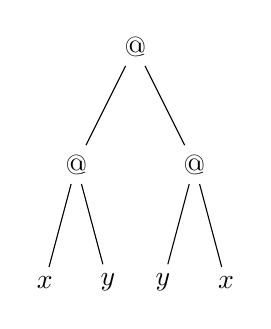
\begin{tikzpicture}
      [level 1/.style={sibling distance=15mm},
        level 2/.style={sibling distance=8mm}]
  \node at (0,0) {@}
  child { node {@}
      child {node {$x$}}
      child { node {$y$} }}
  child { node {@} 
      child {node {$y$}}
      child { node {$x$} }};
 \end{tikzpicture}

  \item

    \

    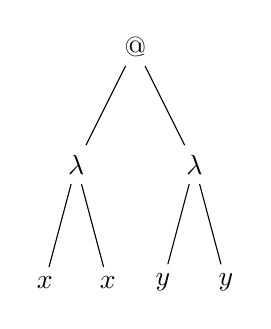
\begin{tikzpicture}
      [level 1/.style={sibling distance=15mm},
        level 2/.style={sibling distance=8mm}]
  \node at (0,0) {@}
  child { node {$\lambda$}
      child {node {$x$}}
      child { node {$x$} }}
  child { node {$\lambda$} 
      child {node {$y$}}
      child { node {$y$} }};
 \end{tikzpicture}


  \item

    \

    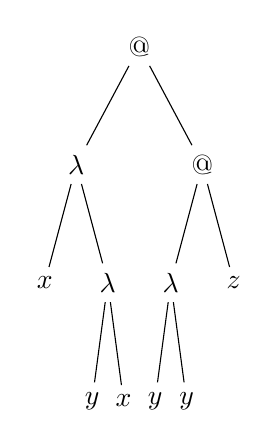
\begin{tikzpicture}
      [level 1/.style={sibling distance=16mm},
        level 2/.style={sibling distance=8mm},
          level 3/.style={sibling distance=4mm}]
  \node at (0,0) {@}
  child { node {$\lambda$}
      child {node {$x$}}
      child { node {$\lambda$}
        child {node {$y$}}
        child {node {$x$}}}}
  child { node {@}
    child { node {$\lambda$} 
        child {node {$y$}}
        child { node {$y$} }}
    child { node {$z$}}};
 \end{tikzpicture}



  \item

    \

    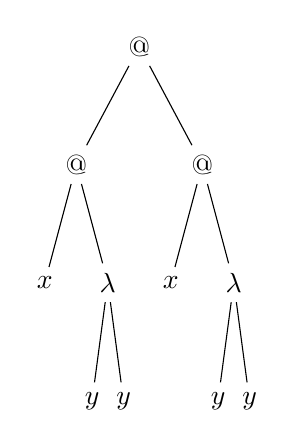
\begin{tikzpicture}
      [level 1/.style={sibling distance=16mm},
        level 2/.style={sibling distance=8mm},
          level 3/.style={sibling distance=4mm}]
  \node at (0,0) {@}
  child { node {@}
      child {node {$x$}}
      child { node {$\lambda$}
        child {node {$y$}}
        child {node {$y$}}}}
  child { node {@}
    child { node {$x$}}
    child { node {$\lambda$} 
        child {node {$y$}}
        child { node {$y$} }}};
 \end{tikzpicture}


  \end{enumerate}


  \end{enumerate}
  
\subsection{Kinds of variable occurrences}

 For each of the given terms, draw them in tree form and then
 indicate, in the same way as in Figure~\ref{fig:varocc}, which
 variable occurrences are binding (please underline), which are bound
 (please circle), and which are free (please box):
\begin{enumerate}

\item $y$

\vspace{.5cm}
\item $\lambda\, y.\ y$

\vspace{.5cm}
\item $(\lambda\, x.\, x\ x)\ y$

\vspace{.5cm}
\item $\lambda\, x.\, (\lambda\, y.\, x)\ y$

\vspace{.5cm}
\item $\lambda\, y.\, \lambda\, z.\, x\ y\ y\ (w\ z)$

\vspace{.5cm}
\end{enumerate}

\subsection{Capture-avoiding substitution}

For each of the following, write the result of the substitution or that it is undefined.

\begin{enumerate}
\item $[x/y]\lam{z}{y\ y}$
  
  \vspace{.5cm}

\item $[(x\ x)/y]\lam{z}{z\ (y\ y)}$

  \vspace{.5cm}

\item $[(x\ x)/y]\lam{y}{z\ y}$

  \vspace{.5cm}

\item $[\lam{x}{x}/y]\lam{z}{y\ \lam{y}{y\ z}}$

  \vspace{.5cm}

\item $[\lam{x}{y}/z]\lam{y}{y\ z}$
  \end{enumerate}


\subsection{Single-step $\beta$-reduction}

\begin{enumerate}
  \item Each of the following reductions is allowed by Definition~\ref{def:betactxt}.  For each reduction, indicate the instantiations of the meta-variables $x$, $t$, $t'$, and $t''$ of Definition~\ref{def:betactxt} (as in the examples in Section~\ref{sec:betaex}).
    \begin{enumerate}
    \item $\lam{x}{(\lam{y}{y})\ \lam{z}{z}}\ \betar \lam{x}{\lam{z}{z}}$
      \vspace{.5cm}
    \item $(\lam{y}{y})\ (z\ z)\ z\ \betar z\ z\ z$
      \vspace{.5cm}
    \item $z\ (\lam{y}{(\lam{z}{z\ z})\ (y\ y)}) \betar z\ \lam{y}{y\ y\ (y\ y)}$
      \vspace{.5cm}
    \item $(\lam{x}{\lam{y}{x\ x}})\ (z\ \lam{z}{z}) \betar \lam{y}{z\ (\lam{z}{z})\ (z\ \lam{z}{z})}$
      \vspace{.5cm}
    \item $(\lam{x}{\lam{y}{y}})\ z \betar \lam{y}{y}$
      \vspace{.5cm}
    \end{enumerate}

  \item Write derivations using the rules of Figure~\ref{fig:betar} for the $\beta$-reductions of parts (a), (b), (c) of the previous problem.

   \end{enumerate}

\subsection{$\alpha$-equivalence}

For each pair of terms, indicate whether or not they are $\alpha$-equivalent:
\begin{enumerate}
\item $\lam{x}{\lam{y}{y\ x}}$ and $\lam{x}{\lam{x}{y\ x}}$
  \vspace{.5cm}
\item $x\ \lam{y}{x}$ and $x\ \lam{w}{x}$
  \vspace{.5cm}
\item $x\ \lam{y}{x}$ and $y\ \lam{x}{y}$
  \vspace{.5cm}
\item $\lam{z}{(\lam{x}{x\ z})\ \lam{y}{z\ y}}$ and $\lam{q}{(\lam{y}{y\ q})\ \lam{y}{q\ y}}$
  \vspace{.5cm}
\end{enumerate}

\subsection{Multi-step $\beta$-reduction}

\begin{enumerate}

\item Write maximal $\curva$-reduction sequences starting with the given term.  Be careful with your renamings!

\begin{enumerate}
\item $\lam{y}{(\lam{x}{\lam{y}{x\ (x\ y)}})\ \lam{x}{y\ x}}$
  \vspace{.5cm}
\item $\lam{x}{\lam{y}{(\lam{z}{\lam{y}{\lam{x}{z\ z}}})\ \lam{z}{x\ y}}}$
  \vspace{.5cm}
\end{enumerate}

% answer: \delta app (in terms of Chapter 2)
\item Find an example of a term $t$ and number $n$ of $\beta$-steps where
  \begin{itemize}
  \item there exists a term $t'$ such that $t (=_\alpha\ \leadsto_\beta^n\ =_\alpha\ \leadsto_\beta) t'$, but
  \item there does not exist a term $t'$ such that $t (=_\alpha\ \leadsto_\beta^{n+1}) t'$.
  \end{itemize}
  \noindent In other words, this problem asks you to find an example of a term where a second $\alpha$-equivalence step is required in order to
  complete a sequence of $\beta$-reductions.  As a hint (because the problem is a bit tricky):
  \begin{itemize}
  \item If all bound and free variables are distinct from each other, then it is never necessary to rename to perform a single $\beta$-reduction, so it might seem like an initial $=_\alpha$-step would suffice to obviate any subsequent renamings... 
    \item ...but it is not! Ask yourself if there is a way that starting with a term where all bound and free variables are distinct from each other, one could arrive at a term that does not have that property; and then use this to construct a term where a second $=_\alpha$-step is required.

  \end{itemize}
\end{enumerate}
